\documentclass[prd,preprintnumbers,twocolumn,eqsecnum,floatfix,a4paper,nofootinbib,superscriptaddress]{revtex4}
\usepackage{color}
\usepackage{calc}
\usepackage{amsmath,amssymb,graphicx}
\usepackage{amssymb,amsmath}
\usepackage{bm}
\usepackage{microtype}
\usepackage{booktabs}
\usepackage{times}
\usepackage[varg]{txfonts}
\usepackage[colorlinks, pdfborder={0 0 0}]{hyperref}
\usepackage[utf8]{inputenc}
\definecolor{LinkColor}{rgb}{0.75, 0, 0}
\definecolor{CiteColor}{rgb}{0, 0.5, 0.5}
\definecolor{UrlColor}{rgb}{0, 0, 0.75}
\hypersetup{linkcolor=LinkColor}
\hypersetup{citecolor=CiteColor}
\hypersetup{urlcolor=UrlColor}
\maxdeadcycles=1000
\allowdisplaybreaks
\textwidth 7 in
\hoffset -0.1in
\textheight 10in
\DeclareFontFamily{OT1}{pzc}{}
\DeclareFontShape{OT1}{pzc}{m}{it}{<-> s * [1.10] pzcmi7t}{}
\DeclareMathAlphabet{\mathpzc}{OT1}{pzc}{m}{it}
\newcommand{\comment}[1]{\textcolor{blue}{\textit{#1}}}
\newcommand{\ajith}[1]{\textcolor{red}{\textit{Ajith:#1}}}
\newcommand{\checkthis}{\textcolor{magenta}{(CHECKTHIS)}}
\newcommand{\vijay}[1]{\textcolor{cyan}{Vijay: #1}}
\newcommand{\io}{\iota}
\newcommand{\p}{\phi}
\newcommand{\vp}{\varphi}

\newcommand{\h}{\mathpzc{h}}
\newcommand{\Hhat}{\hat{\mathpzc{H}}}
\newcommand{\B}{\mathpzc{B}}
\newcommand{\hlm}{\mathpzc{h}_{\ell m}}
\newcommand{\xilm}{\xi_{\ell m}}
\newcommand{\Ylm}{{Y}^{-2}_{\ell m}}
\newcommand{\Y}{{Y}^{-2}}
\newcommand{\hc}{h_\times}
\newcommand{\hp}{h_+}
\newcommand{\Fc}{F_\times}
\newcommand{\Fp}{F_+}
\newcommand{\Mf}{M_f}
\newcommand{\cA}{\mathpzc{A}}
\newcommand{\lm}{_{\ell m}}
\newcommand{\deff}{d_\mathrm{eff}}
\newcommand{\rmi}{\mathrm{i}}
\newcommand{\blambda}{\bm{\lambda}}
\newcommand{\btheta}{\bm{\theta}}
\newcommand{\Mo}{M_{\odot}}
\newcommand{\FFe}{\mathrm{FF}_\mathrm{eff}}
\newcommand{\FF}{\mathrm{FF}}
\newcommand{\e}{\mathrm{e}}
\newcommand{\rhoopt}{\rho_\mathrm{opt}}
\newcommand{\rhosubopt}{\rho_\mathrm{subopt}}
\newcommand{\fqnm}{f}
\newcommand{\sigmaqnm}{\sigma}
\newcommand{\n}{\mathbf{n}}
\newcommand{\bxi}{\bm{\xi}}
\newcommand*{\skymapscale}{0.5}
\newcommand*{\paramestscale}{0.455}

\begin{document}

\newcommand{\be}{\begin{equation}}
\newcommand{\ee}{\end{equation}}
\newcommand{\ber}{\begin{eqnarray}}
\newcommand{\eer}{\end{eqnarray}}
\def\bea{\begin{eqnarray}}
\def\eea{\end{eqnarray}}
\newcommand{\etal}{\emph{et al}}

\title{Accurate inspiral-merger-ringdown gravitational waveforms \\ for non-spinning black-hole binaries including the effect of subdominant modes}
% \author{Ajit Kumar Mehta}
% \affiliation{International Centre for Theoretical Sciences, Tata Institute of Fundamental Research, Bangalore 560012, India}
% \author{Chandra Kant Mishra}
% \affiliation{International Centre for Theoretical Sciences, Tata Institute of Fundamental Research, Bangalore 560012, India}
% \affiliation{Indian Institute of Technology, Madras, Chennai 600036, India}
% \author{Vijay Varma}
% \affiliation{Theoretical Astrophysics, 350-17, California Institute of Technology, Pasadena, CA 91125, USA}
% \affiliation{International Centre for Theoretical Sciences, Tata Institute of Fundamental Research, Bangalore 560012, India}
% \author{Parameswaran~Ajith}
% \affiliation{International Centre for Theoretical Sciences, Tata Institute of Fundamental Research, Bangalore 560012, India}
% \affiliation{Canadian Institute for Advanced Research, CIFAR Azrieli Global Scholar, MaRS Centre, West Tower, 661 University Ave., Suite 505, Toronto, ON M5G 1M1, Canada}

\begin{abstract}
\end{abstract}
\preprint{LIGO-P1700160-v3}
\maketitle
%%%%%%%%%%%%%%%%%%%%%%%%%%%%%%%%%%%%%%%%%%%%%%%%%%%%%%%%%%%%%%%%%%%%%%%%%%%%%%%%%%%%%%%%%%%%%%%%%%%%%%%%%%%%%%%%%%%%%%%%%%%%%%%%%%%%%%%%%%%%%%%`
\section{Introduction}
%%%%%%%%%%%%%%%%%%%%%%%%%%%%%%%%%%%%%%%%%%%%%%%%%%%%%%%%%%%%%%%%%%%%%%%%%%%%%%%%%%%%%%%%%%%%%%%%%%%%%%%%%%%%%%%%%%%%%%%%%%%%%%%%%%%%%%%%%%%%%%%`
\section{Data analysis method}
\subsection{Waveform model}
Gravitational wave radiation emitted by a binary black hole in GR can be written as a linear combination of the `plus' and `cross' polarisations : $\h(t) := h_+(t) - i \, h_\times(t)$, which can be expanded in a basis of spin $-2$ weighted spherical harmonics~\cite{NewmanPenrose} as:
\begin{equation}
\h(t; \n, \blambda, \Delta \blambda)= \frac{1}{d_L} \sum _{\ell=2}^{\infty} \sum _{m=-\ell}^{\ell} {\Ylm} (\n) \, {{\hlm}(t; {\blambda})}, 
\label{eq:spherical_harmonics}
\end{equation}
where ${\Ylm}$ are the basis functions of spin $-2$ spherical harmonics, $\n := \{\iota, \varphi_0\}$ define the direction of radiation in the source frame, $d_L$ is  the luminosity distance to the binary, and ${\h}_{lm}(t; \blambda)$ are the spherical harmonic modes of the waveform. The inclination angle $\iota$ is measured with respect to the orbital angular momentum of the binary. 

The spherical harmonic modes, ${\h}_{lm}(t; \blambda)$, are purely functions of the intrinsic parameters $\blambda$ of the system, while all the angular dependence is captured by the spherical harmonic basis functions ${\Ylm}$.  Here, we consider the black holes to be non-spinning and the binary to be quasi-circular. Hence $\blambda$ consists of only the component masses $m_1$ and $m_2$ of the black holes. However, it is more convenient to use a reparameterization of the mass plane into the \emph{chirp mass} $M_c := {(m_1m_2)^{3/5}}/{(m_1+m_2)^{1/5}}$ and asymmetric mass ratio $q = m_2/m_1 \leq 1$. In GR, the leading contribution in gravitational radiation comes from the quadrupole modes ($\ell = 2, m = \pm 2$). The relative contribution of the higher modes depends on the mass ratio $q$ and the inclination angle $\iota$.  Non-quadrupole modes becomes important when the black holes have significantly unequal masses and larger inclination angle. This multipolar structure (i.e., spherical harmonic modes) of the waveform ${\h}_{lm}(t)$ is completely determined by the set of intrinsic parameters $\blambda := \{M_c, q\}$.

\subsection{Signal model}
The gravitational wave strain observed by a detector can be expressed as
\begin{equation}
h(t) = F_+(\theta, \phi, \psi) \, h_+(t-t_0) + F_{\times}(\theta, \phi, \psi)\, {h}_{\times}(t-t_0), 
\label{eq:det_response}
\end{equation}
where $F_+$ and $F_\times$ are the antenna pattern functions of the GW detector, $t_0$ is the time of arrival of the signal at the detector, and $(\theta, \phi), \psi$ define the source location and polarisation angle of the gravitational wave, respectively. For coalescing BBH systems in quasi-circular orbits, the measured strain $h(t)$ is therefore described by a set of \emph{intrinsic} parameters $\blambda = \{M_c, q\}$ and \emph{extrinsic} parameters  $\btheta := \{t_0, \iota, \varphi_0, d_L, \theta, \phi, \psi\}$ in GR. In addition to the parameters that describe signals in GR, we introduce a set of intrinsic parameters $\Delta \blambda$ and extrinsic parameters $\Delta \btheta$  which captures any possible departure from GR (details in Section \ref{sec3} and Section \ref{sec4}). The deviation parameters $\Delta \blambda$ ($\Delta \btheta$) describes difference between the intrinsic (extrinsic) parameters used to generate the dominant and subdominant modes or the `plus' and `cross' polarizations.  The combined set of parameters is denoted as $\bxi = \{\blambda, \btheta, \Delta \blambda, \Delta \btheta\}$. 

\subsection{Bayesian analysis}
We assume that the data $d(t) = n(t) + h(t)$ from the gravitational wave detector contains both the observed signal $h(t)$ given in Eq.~(\ref{eq:det_response}) and a  stationary Gaussian noise component $n(t)$. Given data $d(t)$, we compute the probability distribution of the combined set of parameters ${\bxi}$ of a paricular hypothesis $H$ associated with a waveform model (details in Section \ref{sec3} and Section \ref{sec4}) using the Bayes theorem: 
\begin{equation}
P({\bxi} \, | \, d, H) = \frac{P({\bxi} \, | \, H) \, P (d \, | \, {\bxi}, H)}{P(d \, | \, H)}.
\label{eq:Bayes_theorem}
\end{equation} 
The \emph{posterior} probability density $P({\bxi}\,|\,d,H)$ that the data contains a signal with parameters $\bxi$ is determined by the \emph{prior} probability distribution $P({\bxi} \, | \, H)$ and the \emph{likelihood} $P (d \, | \, {\bxi}, H)$. Prior $P({\bxi} \, | \, H)$ denotes the probability of the parameters given by the Hypothesis (or signal model). In this paper, the prior density function on the location of the source is  taken  to  be  isotropically  distributed  on  the  sphere of  the  sky,  with
$P({dL} \, | \, H)=d_{L}^{2}$. Furthermore, we use an  isotropic  prior  on  the  orientation  of  the  binary: $P({\iota,\varphi_0,\psi} \, | \, H)=sin\iota$. For all other parameters in $\bxi$, we use uniform prior distribution. The likelihood $P (d \, | \, {\bxi}, H)$ gives the probability of observing data $d(t)$ given the model parameter $\bxi$; and $P(d \, | \, H)$ is a normalization constant, called the \emph{evidence} or the \emph{marginal likelihood}, expressed as:
 \begin{equation}
 P(d \, | \, H)=\int p(d|\bxi)p(\bxi)d\bxi.
 \label{eq:evidence}
 \end{equation}
For stationary Gaussian noise with power spectral density $S_n(f)$, the likelihood is written as:
\begin{equation}
P (d \, | \, {\bxi}, H) = \text{exp}\left[ -\frac{1}{2}\int_{f_\mathrm{low}}^{f_\mathrm{high}} \frac{|\tilde{d}(f) - \tilde{h}(f;{\bxi}, H)|^2}{S_n(f)}df\right],
\end{equation}
where $\tilde{d}(f)$ and $\tilde{h}(f)$ are the Fourier transforms of $d(t)$ and $h(t)$, respectively. The limits of the integration $f_\mathrm{low}$ and $f_\mathrm{high}$ define the sensitivity bandwidth of the detector. In this work, we use a network of three LIGO-VIRGO detectors. We assume that the noise is uncorrelated in each detector. The network likelihood for data obtained from three detectors can thus be written as the product of the likelihoods in each detector
\begin{equation}
P (d \, | \, {\bxi}, H, S_n(f)) = \prod_{i \epsilon {H,L,V}} P (d_{i} \, | \, {\bxi}, H, S_{n_{i}}(f)).
\end{equation}

Using the Bayesian framework described above, we estimate $\bxi$ by stochastically sampling over the entire parameter space of interest. We use python-based affine-invariant ensemble sampler \texttt{emcee}~\cite{foreman2013emcee} for Markov chain Monte Carlo (MCMC) proposed by \cite{goodman2010ensemble} to obtain the posterior distribution $P(\bxi \, | \, d, H)$ of the full parameter set. Posterior distributions of particular parameters of interest, for example,  the set of parameters ${\Delta \blambda, \Delta \btheta}$, describing deviation from the GR prediction of a BBH signal, are computed  by marginalizing the posterior over all other parameters $\{\blambda, \btheta\}$. If the data is consistent with a BBH signal in GR, we expect $P(\Delta \blambda \, | \, d, H)$ to be consistent with zero. 

\subsection{Constraining deviation parameters  using GR waveforms}
We employ the recent phenomenological inspiral-merger-ringdown waveform model proposed by~\cite{Mehta:2017jpq}, which provide accurate Fourier-domain models of three sub-dominant spherical harmonic modes ($(\ell = 2, m=\pm1)$, $(\ell = 3, m=\pm3)$, $(\ell = 4, m = \pm4)$) apart from the dominant $(\ell = 2, m = \pm2)$ mode of the expected GW signals from non-spinning BBHs. The other spherical harmonic modes neglected in this work only introduce an inaccuracy (mismatch) of less than 1\% in the waveforms~\cite{Mehta:2017jpq}. We combine these signals with stationary Gaussian noise with power spectral density anticipated in Advanced LIGO's ``high-power, zero-detuning'' configuration~\cite{aLIGOZeroDetHighPower}, making use of Eqs.~(\ref{eq:spherical_harmonics}) and (\ref{eq:det_response}), and simulate GR observations. We consider binaries with total mass $M := m_1 + m_2$ in the range $40 M_\odot$ -- 200 $M_\odot$ with mass ratio $q := m_2/m_1$ in the range 1/9 -- 1, with varying inclination angles $\iota=\{30^{\circ},45^{\circ},60^{\circ},80^{\circ},90^{\circ}\}$. Using these simulated GR events, we compute the marginalized posterior distribution of the deviation parameters  $\{\Delta \blambda, \Delta \btheta\}$. In order to compute the constraints on these parameters, we calculate the 90\% probability interval. Parameters which are recovered with greatest precision from the simulated GR signal will result smaller values for the credible interval and therefore would give more stringent test of GR with actual observation.

%%%%%%%%%%%%%%%%%%%%%%%%%%%%%%%%%%%%%%%%%%%%%%%%%%%%%%%%%%%%%%%%%%%%%%%%%%%%%%%%%%%%%%%%%%%%%%%%%%%%%%%%%%%%%%%%%%%%%%%%%%%%%%%%%%%%%%%%%%%%%%%`
\section{Consistency between spherical harmonic modes}
\label{sec3}
In this section, we present two tests of GR based on checking the consistency between different spherical harmonic modes of the observed signal. Our strategy, developed below, is to introduce extra parameters in the higher order modes of radiation, both intrinsic and extrinsic, that describe inconsistency between different modes and to constrain them using a Bayesian framework. 

\subsection{Consistency between parameters estimated from different modes}
The first test we consider broadly follows the outline presented in ~\cite{dhanpal2018} to check for the consistency of intrinsic parameters $\blambda := \{M_c, q\}$ estimated from the dominant mode and the higher order modes. According to this, we would estimate the chirp mass and asymmetric mas ratio of the BBH from the leading quadrapolar mode of the observed signal. Independently, we would obtain the same estimates from the higher order modes. In GR, these two estimates of $M_c$ and $q$ should match. 

The test is formulated in the following way: we rewrite Eq.~(\ref{eq:spherical_harmonics}) by splitting the contributions from the dominant $(\ell = 2, m = \pm 2)$ mode of gravitational radiation, and the sub-dominant (higher order) modes 
\begin{eqnarray}
\h(t; \n, \blambda, \Delta \blambda) & = & \sum_{m = \pm2} Y^{-2}_{2m} (\n) {\h}_{2m}(t, \blambda)  \nonumber \\ 
& + & \sum _{\text{H.O.M}} \Ylm (\n) \hlm(t, \blambda+\Delta \blambda)
\label{eq:test_HM}
\end{eqnarray}
where the sum in the second term on the RHS is just over the higher-order modes and incorporate a deviation $\Delta \blambda := \{\Delta M_c, \Delta q\}$ in the set of intrinsic parameters that describe the higher order modes. In the absence of any departure from GR, we expect $\Delta \blambda $ to be consistent with zero. While ~\cite{dhanpal2018} fouces on one performing this test with only one arbitrary detector, we generalize the test in realistic three detector LIGO-VIRGO setup.

%%%%%%%%%%%%%%%%%%%%%%%%%%%%%%%%%%%%%%%%%%%%%%%%%%%%%%%%%%%%%%%%%%%%%%%%%%%%%%%%%%%%%%%%%%
\begin{figure}[htb] \begin{center}
		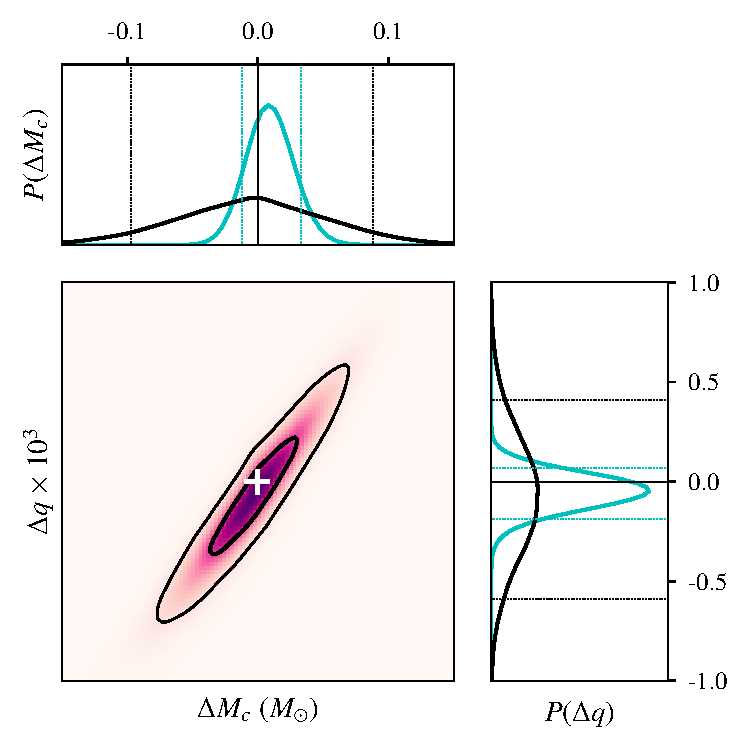
\includegraphics[width=3.4in]{figs/hm_mcq_GR.pdf}
		\caption{(\textbf{Middle panel}): the thick (thin) contours show the 50\% (90\%) credible regions in the joint posteriors of two parameters $\Delta M_c$ and $\Delta q$ that describe deviations in the estimated parameters using the quadrupole and non-quadrupole modes, estimated from a simulated GR signal. (\textbf{Side panels}): Black histograms show the 2-dimensional marginalized posteriors in $\Delta M_c$ and $\Delta q$, while the cyan histograms show the 1-dimensional posteriors in $\Delta M_c$ and $\Delta q$ estimated from the data by introducing only one deviation parameter (say, $\Delta M_c$) at a time, keeping the other fixed (say, $\Delta q = 0$). The posteriors are fully consistent with the GR prediction of $\Delta M_c = \Delta q = 0$ (shown by a ``+'' sign in the center panel and by thin black lines in side panels). The dotted lines mark the 90\% credible regions. The simulated GR signal corresponds to a binary with total mass $M = {80}M_\odot$ and mass ratio $q = 1/9$ and an inclination angle $\iota = {60^\circ}$ observed by Advanced LIGO-VIRGO detectors network with an optimal SNR of 25. }
		\label{fig:posterior_BBH_GR_inj}
\end{center} \end{figure}
%%%%%%%%%%%%%%%%%%%%%%%%%%%%%%%%%%%%%%%%%%%%%%%%%%%%%%%%%%%%%%%%%%%%%%%%%%%%%%%%%%%%%%%%%%

We consider two different ways to perform the test. First, we introduce \emph{one} deviation parameter at a time. That is, $\Delta\blambda = {\Delta M_c}$ or $\Delta\blambda = {\Delta q}$. We then consider introducing a concurrent deviation in \emph{two} parameters $\Delta \blambda = \{\Delta M_c, \Delta q\}$. In Fig. 
~\ref{fig:posterior_BBH_GR_inj}, we show the results of the tests performed with GR waveform by varying either one parameter or two parameters, for a binary with total mass $M = 80M_{\odot}$, mass ratio $q=1/9$, inclination angle $ {\iota}=60^{\circ} $ producing a signal-to-noise ratio  (SNR)  of 25 (SNR in higher modes is $\sim 10$). The posterior probability density for both the parameters $\Delta q$ and $\Delta M_c$ are consistent with zero as one expect in GR. Furthermore, the deviation parameters are found to be better constrained when only one deviation parameter is allowed to vary at a time (either $\Delta M_c$ or $\Delta q$). This suggests that a consistency test with only one deviation parameter in the higher modes would allow a more efficient test. In the subsequent analysis, we therefore focus on varying only one deviation parameter at a time. 

Up next, in Fig. \ref{fig:hm_mcq_compare-1det_3det_GR_inj} we show that, as expected, the width of the posteriors of the deviation parameters become smaller when we perform the test with a network of three Advanced LIGO-VIRGO detectors instead of using only one Advanced LIGO detector. 

 

%%%%%%%%%%%%%%%%%%%%%%%%%%%%%%%%%%%%%%%%%%%%%%%%%%%%%%%%%%%%%%%%%%%%%%%%%%%%%%%%%%%%%%%%%%
\begin{figure}[htb] \begin{center}
		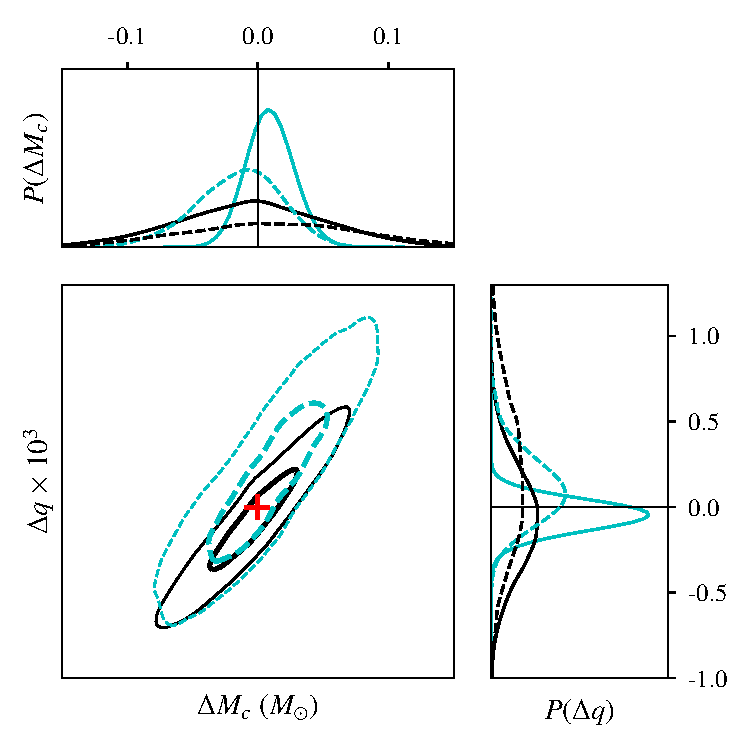
\includegraphics[width=3.4in]{figs/hm_mcq_1det_3det_compare_GR.pdf}
		\caption{(\textbf{Middle panel}): the thick (thin) contours show the 50\% (90\%) credible regions in the joint posteriors of two parameters $\Delta M_c$ and $\Delta q$ that describe deviations in the estimated parameters using the quadrupole and non-quadrupole modes, estimated from a simulated GR signal. Solid black lines indicates the joint posterior obtained by network of three detectors in Advanced LIGO-VIRGO setup, while dashed cyan lines show the  joint posterior obtained with only one Advanced LIGO detector. (\textbf{Side panels}): Black histograms show the 2-dimensional marginalized posteriors in $\Delta M_c$ and $\Delta q$, while the cyan histograms show the 1-dimensional posteriors in $\Delta M_c$ and $\Delta q$ estimated from the data by introducing only one deviation parameter (say, $\Delta M_c$) at a time, keeping the other fixed (say, $\Delta q = 0$). The posteriors are fully consistent with the GR prediction of $\Delta M_c = \Delta q = 0$ (shown by a ``+'' sign in the center panel and by thin black lines in side panels).  Solid lines indicates the posterior recovered by network of three detectors in Advanced LIGO-VIRGO setup and dashed lines implies the posterior obtained with only one Advanced LIGO detector. The simulated GR signal corresponds to a binary with total mass $M = {80}M_\odot$ and mass ratio $q = 1/9$ and an inclination angle $\iota = {60^\circ}$ observed either by one Advanced LIGO detector or network of LIGO-VIRGO detectors with an optimal SNR of 25. }
		\label{fig:hm_mcq_compare-1det_3det_GR_inj}
	\end{center} \end{figure}
	%%%%%%%%%%%%%%%%%%%%%%%%%%%%%%%%%%%%%%%%%%%%%%%%%%%%%%%%%%%%%%%%%%%%%%%%%%%%%%%%%%%%%%%%%%
 Figures~\ref{fig:delmc_delq_varyingM} and \ref{fig:delmc_delq_varyingq} show the 90\% credible intervals of the posteriors of the deviation parameters for binaries with varying masses, mass ratios and inclination angles. In all cases, we set the SNR to be {25}.  We find that binaries with large mass ratios ($q < 1/ 2$) and inclination angles ($\iota > 60 ^\circ $) will allow precision tests of the GR predictions, reaching statistical uncertainties of $< 10^{-3}$ for $\Delta q$ and $< 10^{-2}$ for the dimensionless deviation parameter $\Delta M_c/M_c$. We note that the 90\% interval for both the deviation parameters decreases slightly compared to the earlier reported values in~\cite{dhanpal2018}.
 
 \begin{figure}[tbh]
 	\begin{center}
 		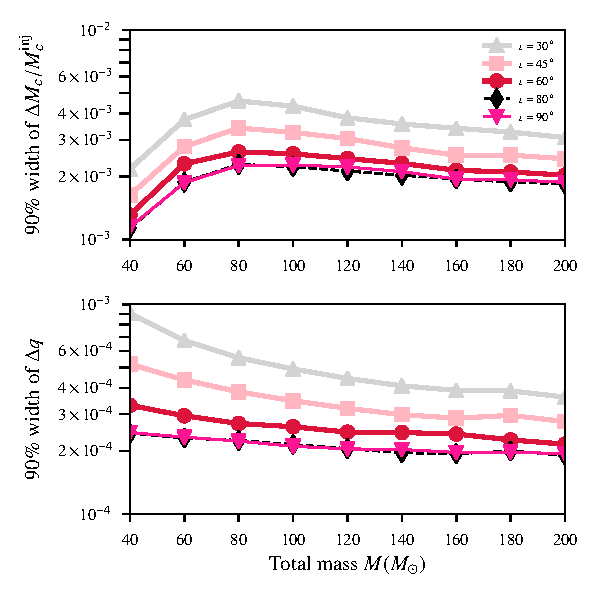
\includegraphics[scale=0.8]{figs/hm_9dim_dmcbymcinj_dq_diff_M.pdf}
 	\end{center} 
 	\caption{The figure shows the width of the 90$\%$ confidence limit of the deviation parameters $\Delta M_c$ and $\Delta q$ for binaries with different total mass (horizontal axis) and inclination angles $\iota$ (legends). All binaries have an asymmetric mass ratio $q=1/9$.}
 	\label{fig:delmc_delq_varyingM}
 \end{figure}
 
 \begin{figure}[tbh]
 	\begin{center}
 		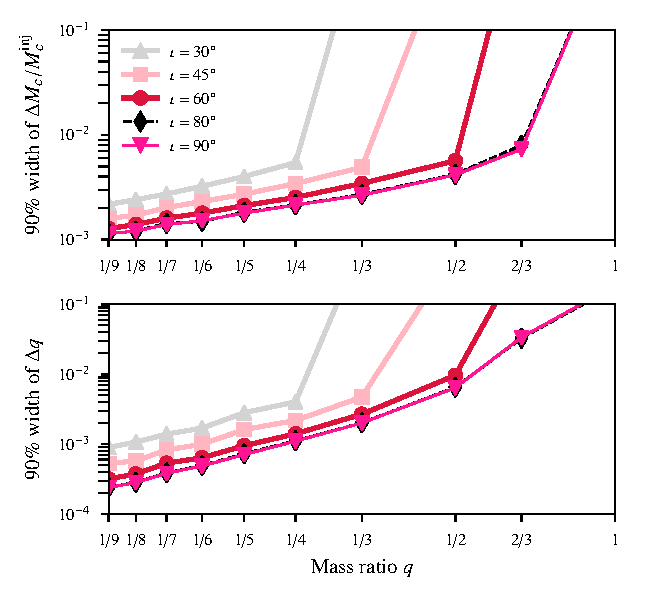
\includegraphics[scale=0.8]{figs/hm_9dim_dmcbymcinj_dq_diff_q.pdf}
 	\end{center} 
 	\caption{Same as Fig.~\ref{fig:delmc_delq_varyingM}, except that the horizontal axis reports the mass ratio $q$. All binaries correspond to a total mass $40M_{\odot}$.}
 	\label{fig:delmc_delq_varyingq}
 \end{figure}
%%%%%%%%%%%%%%%%%%%%%%%%%%%%%%%%%%%%%%%%%%%%%%%%%%%%%%%%%%%%%%%%%%%%%%%%%%%%%%%%%%%%%%%%%%%%%%%%%%%%%%%%%%%%%%%%%%%%%%%%%%%%%%%%%%%%%%%%%%%%%%%`

\newpage
\subsection{Consistency between the amplitude and phase from different modes}
We split the contributions from the dominant $(\ell = 2, m = \pm 2)$ mode of gravitational radiation, and the higher order modes 
\begin{eqnarray}
{\h}(t; n, \blambda, \Delta \blambda) & = & \sum_{m = \pm2} Y^{-2}_{2m} (n) {\h}_{2m}(t, \blambda)  \nonumber \\ 
& + & \sum _{\text{H.O.M}} (1+\Tilde{c_1})\Ylm (n) \hlm(t, \blambda)
\label{eq:test_amp}
\end{eqnarray}
where  H.O.M represents the higher order modes, and $\blambda$ the intrinsic parameters (say, chirp mass $M_c$ and mass ratio $q$). We introduce a deviation parameter $\Tilde{c_1}$ in H.O.M amplitudes, where $\Tilde{c_1}$ is complex in nature. We estimate $\Tilde{c_1}$ in addition to the standard set of intrinsic and extrinsic parameters in general relativity (GR). $\Tilde{c_1}$ would be zero for GR.

\newpage 
\noindent Corner plot  - Fig \ref{fig:c1_corner};\\
triangle plot - Fig \ref{fig:c1_triangle};\\
90\% credible intervals of $\Tilde{c_1}$  - Fig \ref{fig:c1_bound_a}, Fig \ref{fig:c1_bound_b} \& Fig \ref{fig:c1_bound_c}
\newpage

\begin{figure}[tbh]
\begin{center}
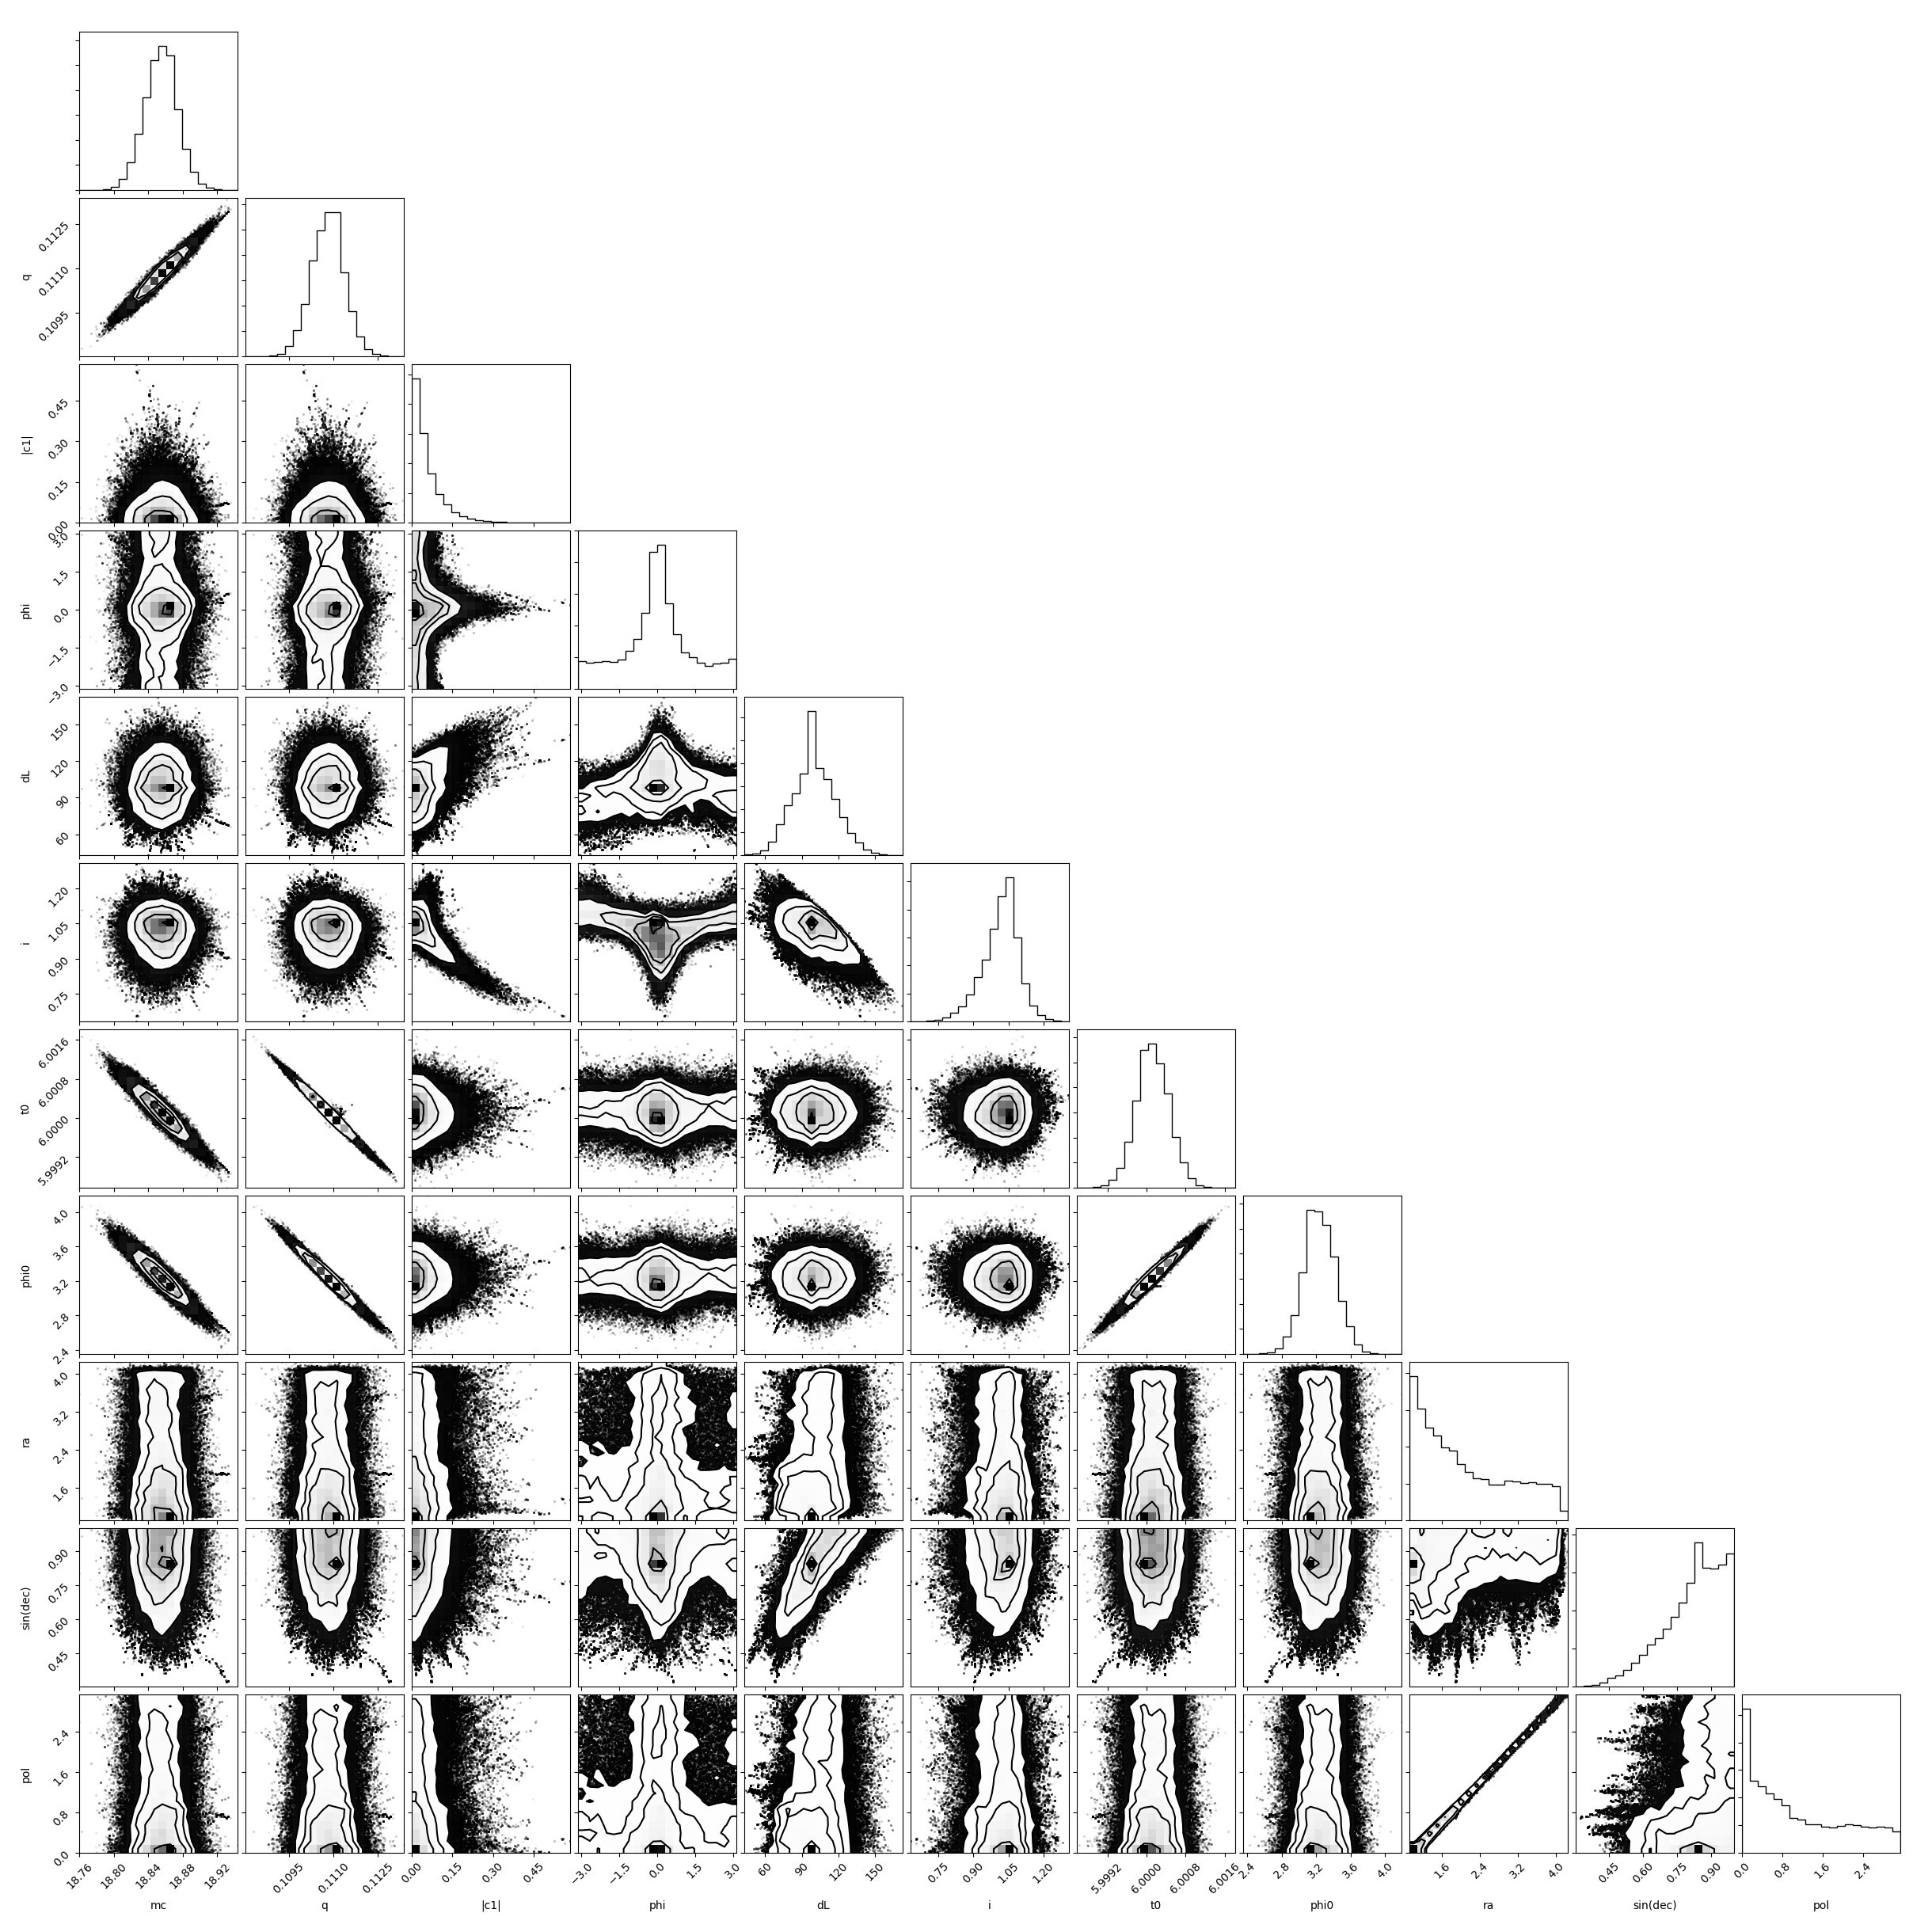
\includegraphics[scale=0.25]{figs/c1_80_9_100_corner_plot_wo_burnin.png} 
\end{center} 
\caption{Corner plot for tests of GR with complex deviation parameter $c_1$ in the higher order modes. M=80, q=9 and SNR=100.}
\label{fig:c1_corner}
\end{figure}

\newpage
.
\newpage 


\begin{figure}[tbh]
    \begin{center}
    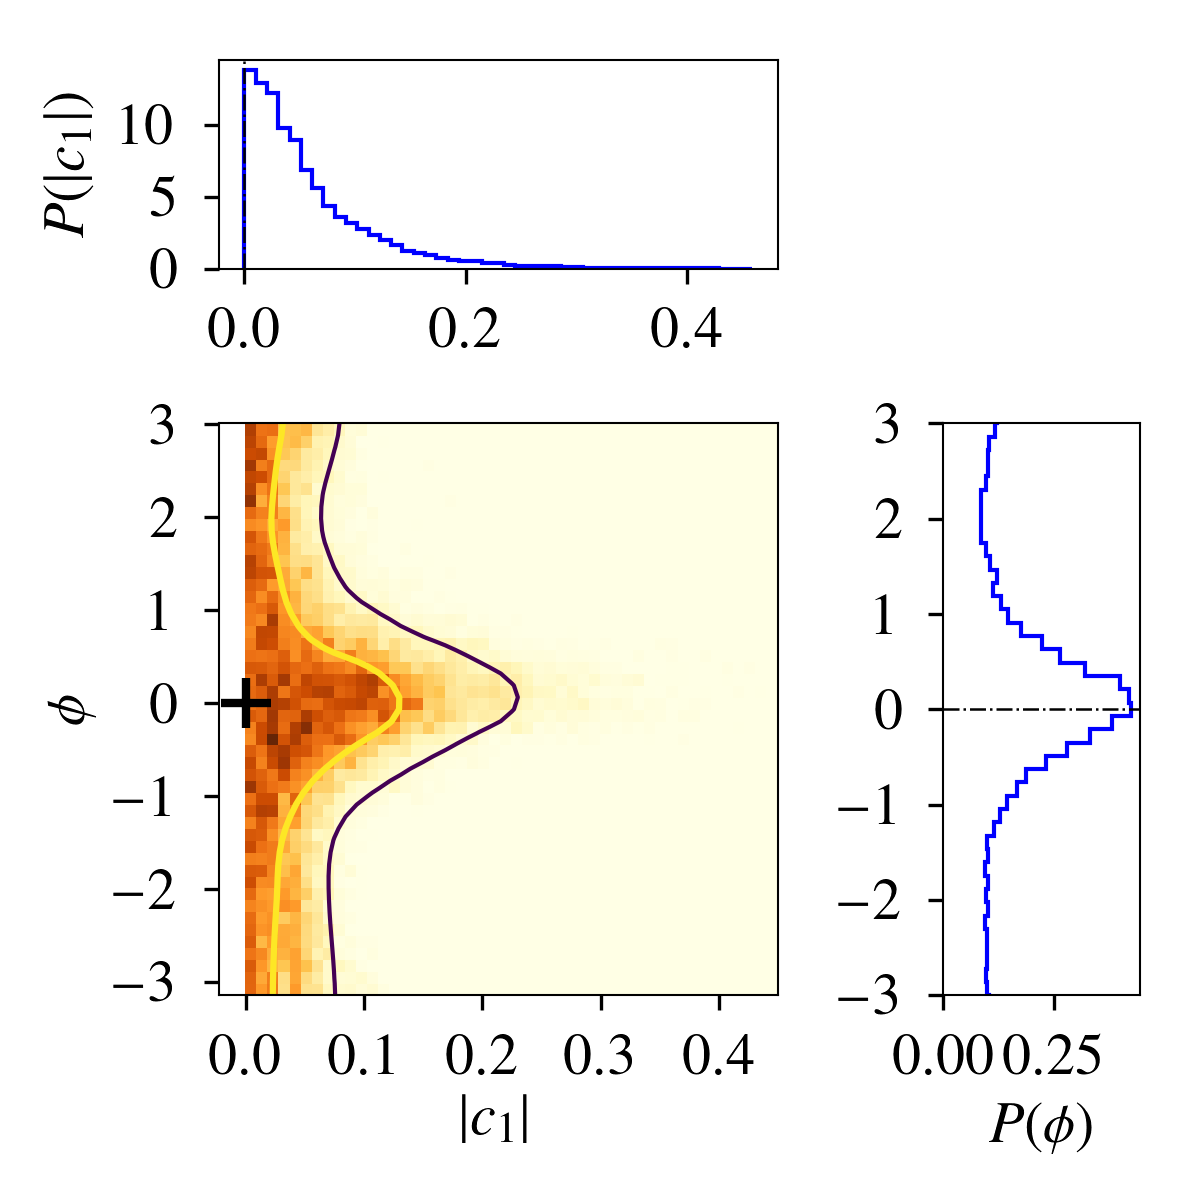
\includegraphics[scale=0.8]{figs/triangle_plot_M_80_q_9_snr_100_complex_c1.png}
    %
\includegraphics[scale=0.75]{figs/triangle_plot_M_80_q_9_snr_100_complex_c1.pdf}
    \end{center} 
    \caption{The middle plot shows the 50\% and 90\% credible regions in joint posteriors of two parameters: amplitude $|c_1|$ and phase $\phi$ of the complex deviation parameter $c_1$ estimated from different simulated GR signal corresponding to a binary with total mass $M=80$ $M_{\odot}$ , mass ratio $q=9$ and SNR 100.}
    \label{fig:c1_triangle}
\end{figure}

\begin{figure}[h]
    \begin{center}
    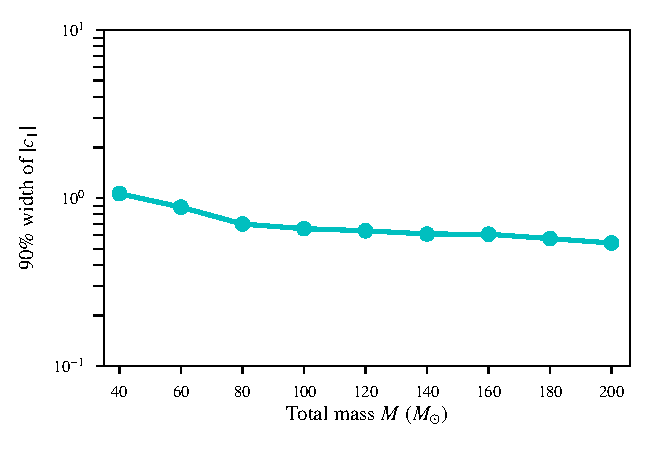
\includegraphics[scale=0.75]{figs/confidence_interval_c1_varying_M_q_9_snr_25.pdf} 
    \end{center} 
    \caption{The plots shows the width of the 90\% credible region of $|c_1|$ as a function of total mass $M$. All binaries correspond to a mass ratio $q = 1/9$ and SNR 25.}
    \label{fig:c1_bound_a}
\end{figure}

\begin{figure}[h]
    \begin{center}
    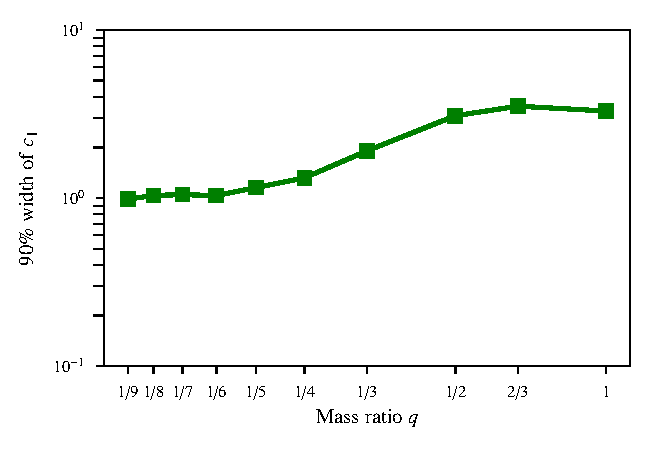
\includegraphics[scale=0.75]{figs/confidence_interval_c1_varying_q_M_40_snr_25.pdf} 
    \end{center} 
    \caption{The plots shows the width of the 90\% credible region of $|c_1|$ as a function of mass ratio $q$. All binaries correspond to a mass ratio $M = 40$ $M_{\odot}$ and SNR 25.}
    \label{fig:c1_bound_b}
\end{figure}

\newpage
\begin{figure}[h]
    \begin{center}
    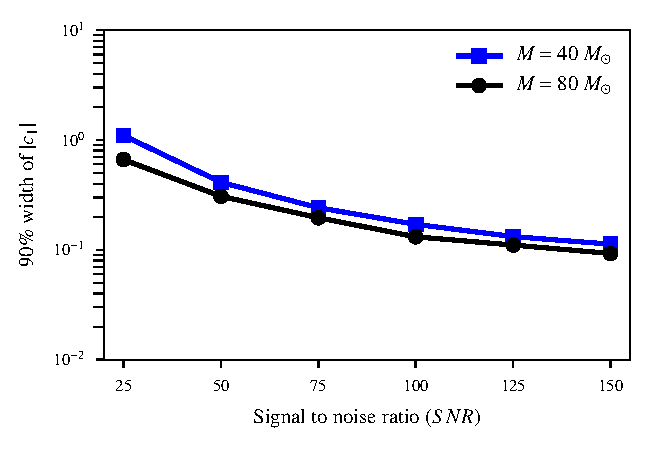
\includegraphics[scale=0.75]{figs/confidence_interval_c1_varying_snr.pdf} 
    \end{center} 
    \caption{The plots shows the width of the 90\% credible region of of $|c_1|$ as a function of signal to noise ratio. All binaries correspond to a mass ratio $q = 1/9$. Total mass $M={40,80}$ $M_{\odot}$.}
    \label{fig:c1_bound_c}
\end{figure}

%%%%%%%%%%%%%%%%%%%%%%%%%%%%%%%%%%%%%%%%%%%%%%%%%%%%%%%%%%%%%%%%%%%%%%%%%%%%%%%%%%%%%%%%%%%%%%%%%%%%%%%%%%%%%%%%%%%%%%%%%%%%%%%%%%%%%%%%%%%%%%%`
\newpage
\section{Consistency between polarizations}
\label{sec4}
\subsection{Consistency between parameters estimated from different polarizations}

We allow the possibility of inconsistency between the polarization states $h_+$ and $h_\times$ by introducing deviation parameters  $\Delta \blambda := \{\Delta M_c, \Delta q\}$ in the set of intrinsic parameters for $h_\times$.
\begin{eqnarray} 
\h(t; \blambda, \Delta \blambda) =  h_+(t; \blambda) - ih_\times(t; \blambda, \Delta \blambda)
\label{eq:test_hp_hc}
\end{eqnarray}
We estimate these additional parameters $\Delta \blambda$ in addition to the standard set of parameters in GR. Note that $\Delta \blambda = \{0,0\}$ in GR.

\newpage 
\noindent Corner plot  - Fig \ref{fig:hphc_corner};\\
triangle plot - Fig \ref{fig:hphc_triangle};\\
90\% credible intervals of $\Delta$ $M_{c}$ and $\Delta$ $q$  - Fig \ref{fig:hphc_bound_a}, \& Fig \ref{fig:hphc_bound_b};

\newpage

\begin{figure}[htb]
    \begin{center}
    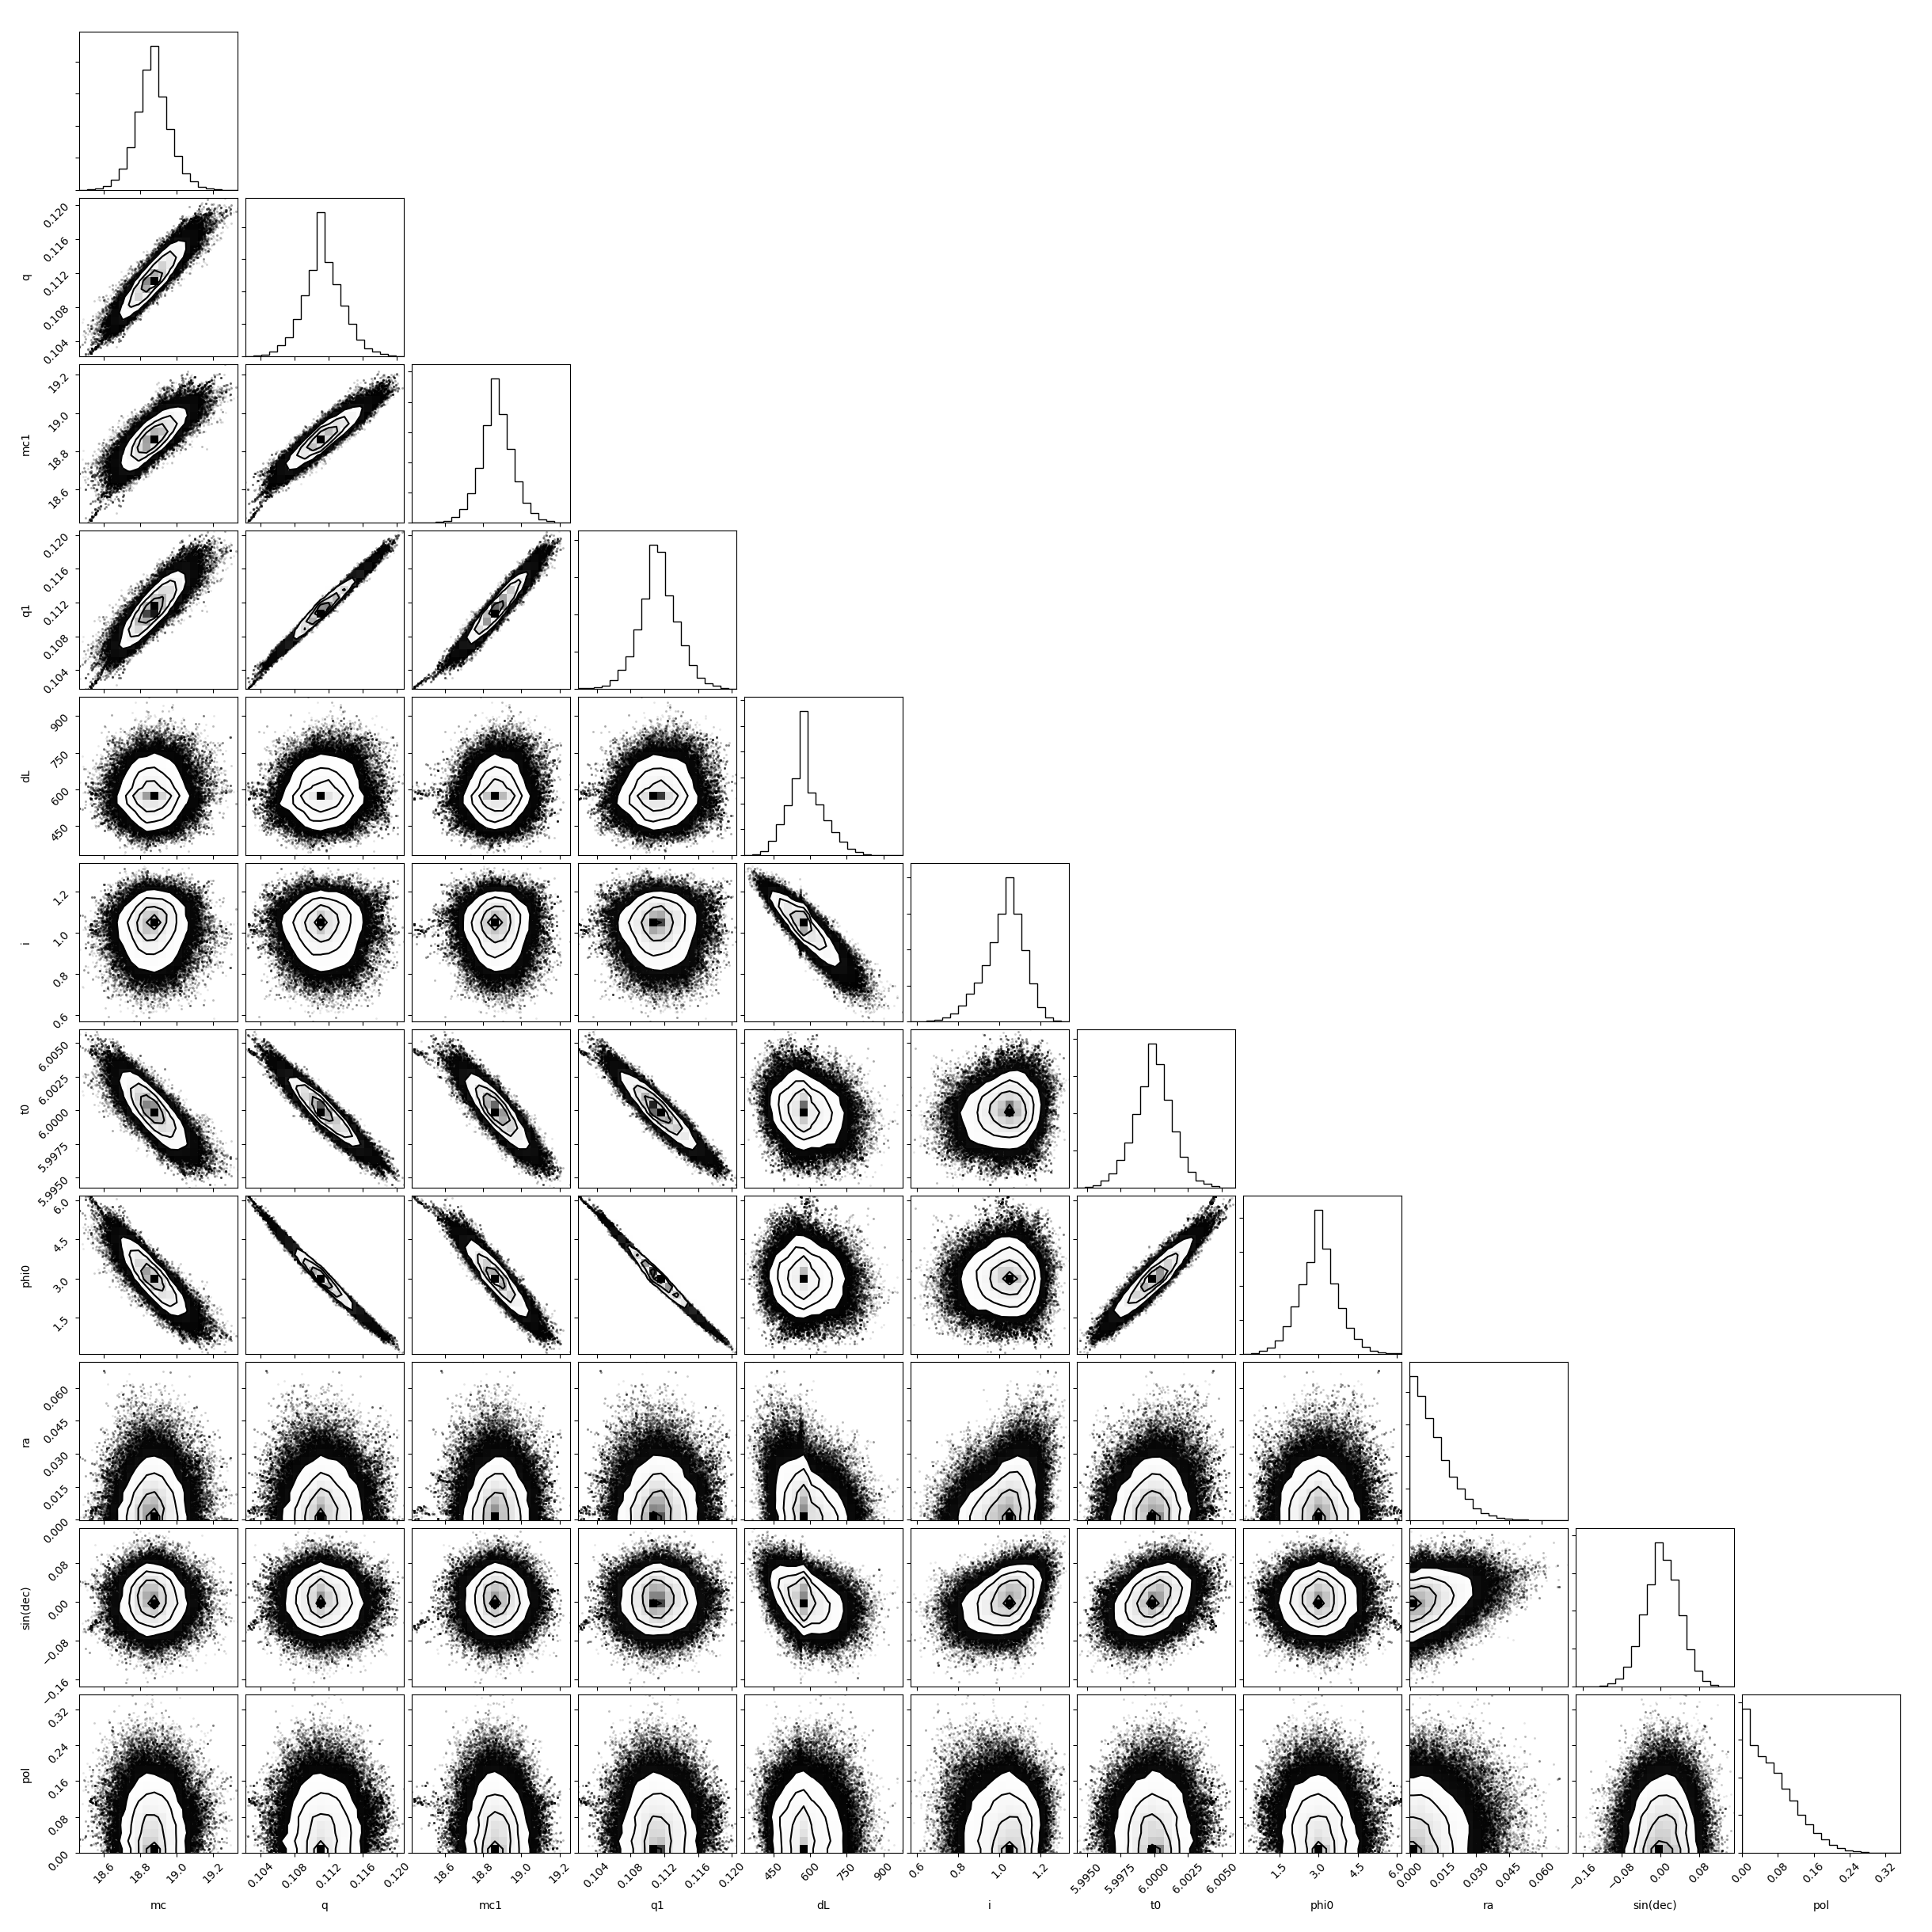
\includegraphics[scale=0.3]{figs/hp_hc_consistency_polarization_corner_plot_M_80_q_9_snr_25.png} 
    \end{center} 
    \caption{Corner plot for tests of GR based on checking for consistency between parameters ($M_{c}$, $q$, 
    $\Delta$ $M_{c}$ and $\Delta$ $q$) estimated from different polarizations. }
    \label{fig:hphc_corner}
\end{figure}

\newpage
.
\newpage

\begin{figure}[h]
    \begin{center}
    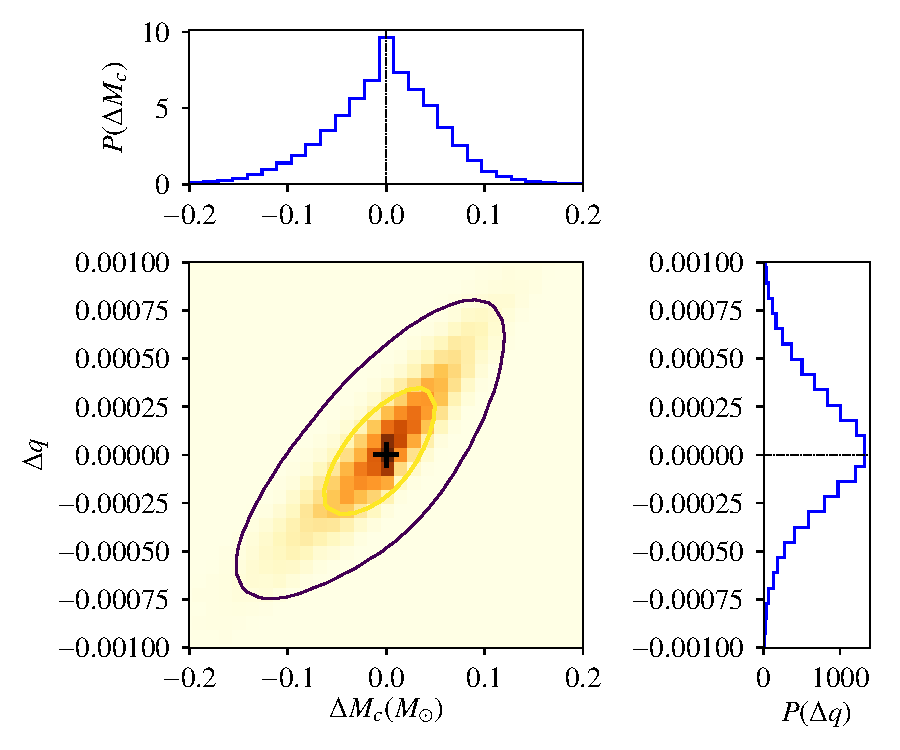
\includegraphics[scale=0.55]{figs/hp_hc_consistency_triangle_plot_delMc_delq_M_80_q_9_snr_25_pol.pdf} 
    \end{center} 
    \caption{The middle plot shows the 68\% and 95\% credible regions in joint posteriors of two parameters $\Delta$ $M_{c}$ and $\Delta$ $q$ estimated from different polarizations of simulated GR signal corresponding to a binary with total mass $M=80$ $M_{\odot}$ , mass ratio $q=9$ and SNR 25.}
    \label{fig:hphc_triangle}
\end{figure}

\begin{figure}[h]
    \begin{center}
    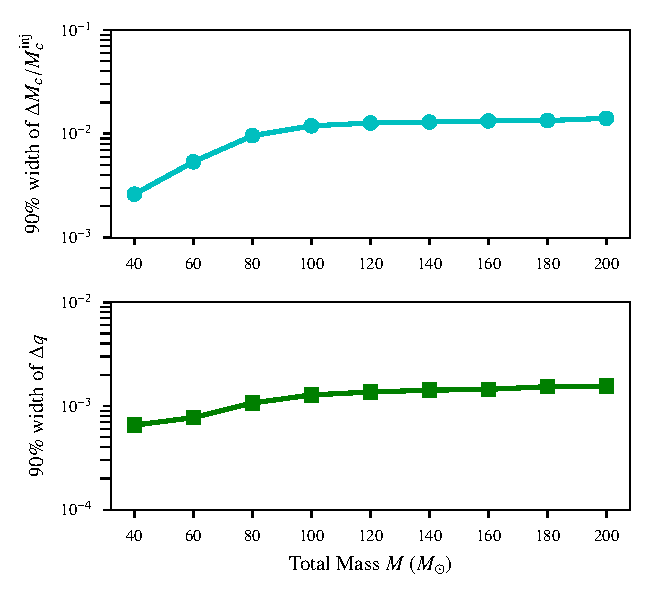
\includegraphics[scale=0.75]{figs/hp_hc_consistency_confidence_interval_varying_M.pdf} 
    \end{center} 
    \caption{The plots shows the width of the 90\% credible region of the $\Delta$ $M_{c}$ and $\Delta$ $q$ estimated from different polarizations of simulated GR signals for binaries with different total mass $M$. All binaries correspond to a mass ratio $q = 1/9$ and SNR 25.}
    \label{fig:hphc_bound_a}
\end{figure}

\newpage

\begin{figure}[]
    \begin{center}
    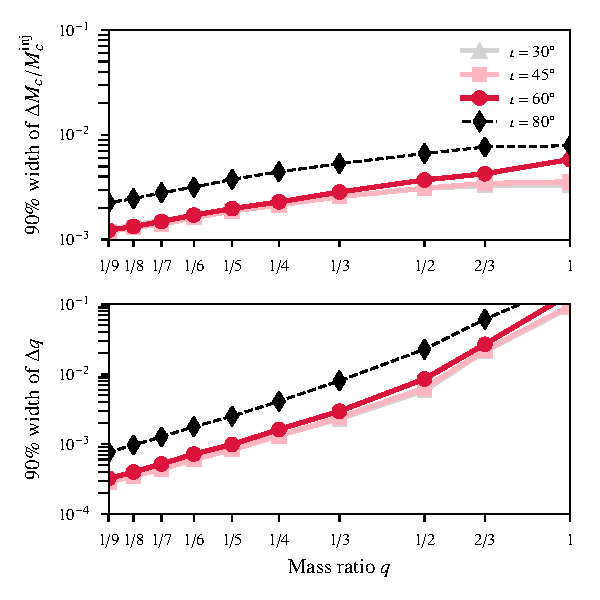
\includegraphics[scale=0.75]{figs/hp_hc_consistency_confidence_interval_varying_q.pdf} 
    \end{center} 
    \caption{The plots shows the width of the 90\% credible region of the $\Delta$ $M_{c}$ and $\Delta$ $q$ estimated from different polarizations of simulated GR signals for binaries with different total mass ratio $q$. All binaries correspond to a mass ratio $M=40$ $M_{\odot}$ and SNR 25.}
    \label{fig:hphc_bound_b}
\end{figure}


%%%%%%%%%%%%%%%%%%%%%%%%%%%%%%%%%%%%%%%%%%%%%%%%%%%%%%%%%%%%%%%%%%%%%%%%%%%%%%
\newpage

\subsection{Consistency between the amplitude of different polarizations}
\subsubsection{$v(f) = v$}
required (?)
\subsubsection{$v(f) = v f$}
In GR, the gravitational radiation could be written as a complex time series $\h(t)=h_+(t) - ih_\times(t)$. However, due to birefringence, one of the polarization can get amplified while the other one may get damped. We formulate a test for amplitude birefringence by introducing a coupling parameter $v$:
\begin{eqnarray} 
\h(f; \blambda) =  \Hat{h_+}(f; \blambda) - i \Hat{h_\times}(f; \blambda),
\label{eq:test_cs}
\end{eqnarray}
where $\Hat{h_+}(f; \blambda)=h^{GR}_+ + i v f h^{GR}_{\times}$ and $\Hat{h_\times}(f; \blambda)=h^{GR}_\times - i v f h^{GR}_{+}$.
Corner plot  - Fig \ref{fig:cs_corner};\\
triangle plot - Fig \ref{fig:cs_hist};\\
90\% credible intervals of $v$  - Fig \ref{fig:cs_bound};\\
modGR injection - Fig \ref{fig:cs_modgr};

\newpage

\begin{figure}[h!]
    \begin{center}
    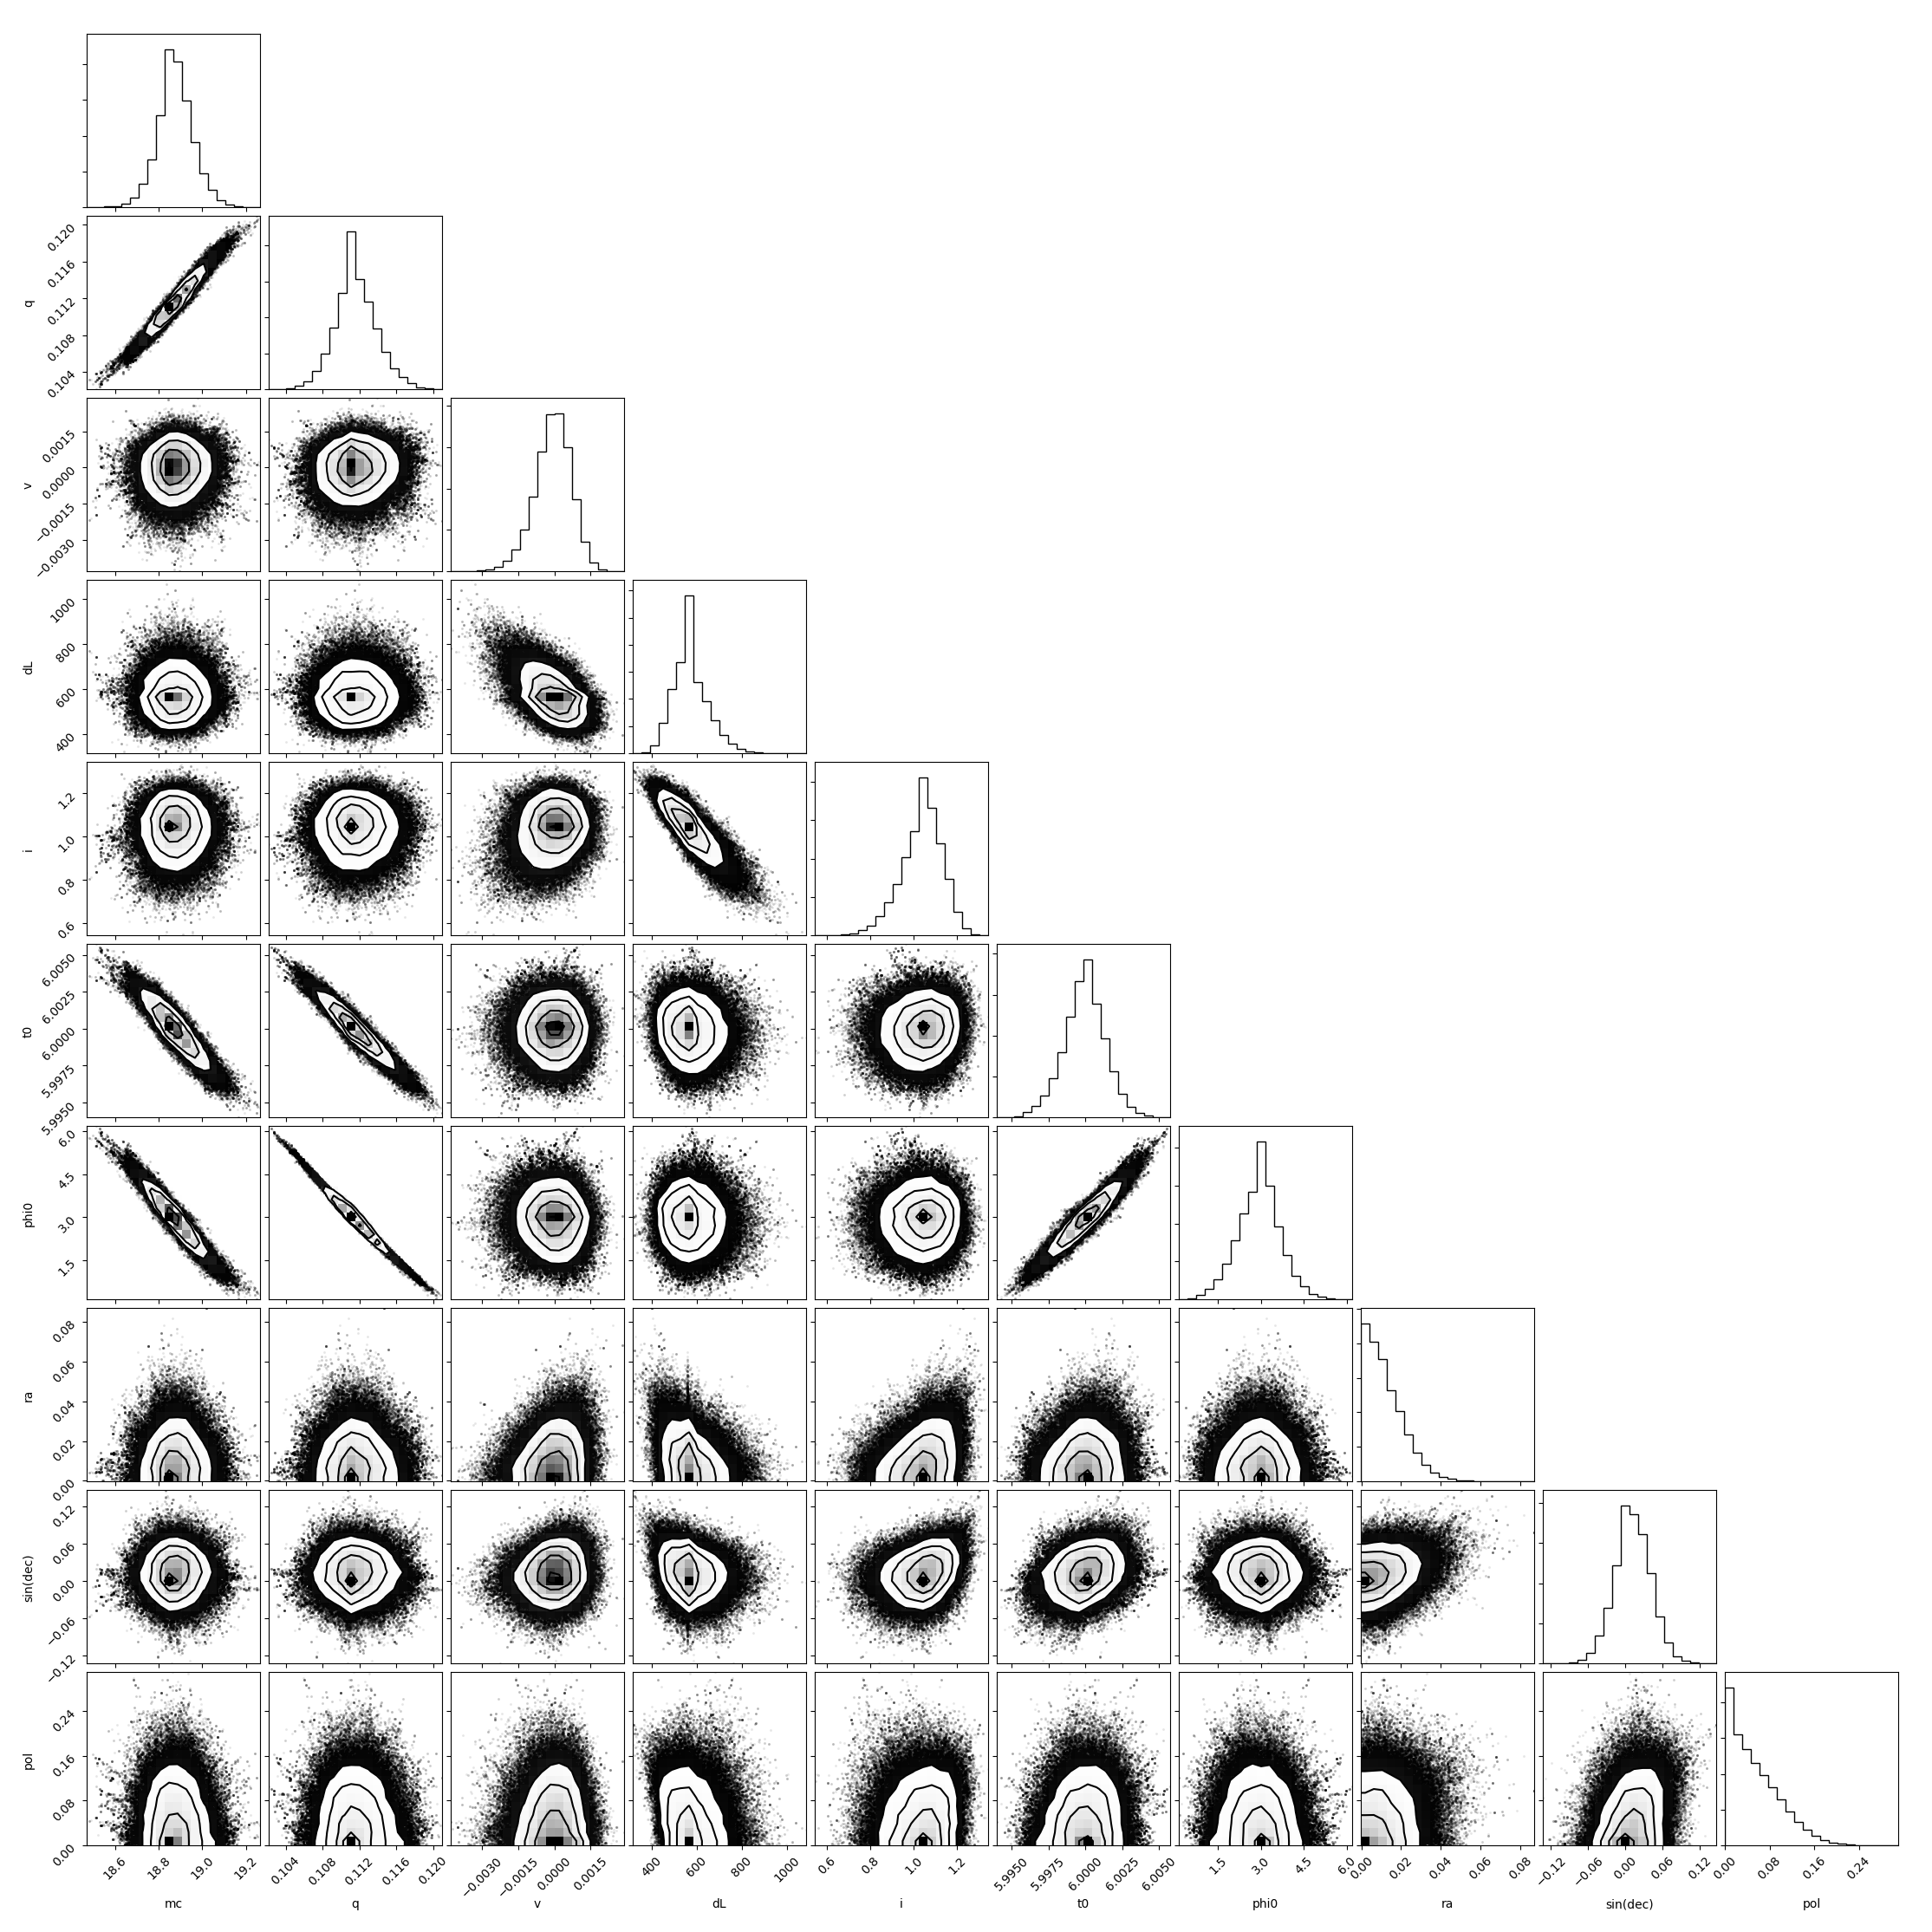
\includegraphics[scale=0.3]{figs/v1_80925_corner_plot.png} 
    \end{center} 
    \caption{Corner plot for tests of GR based on checking consistency between the amplitude of different polarization.}
    \label{fig:cs_corner}
\end{figure}

\newpage
.
\newpage

\begin{figure}[h!]
    \begin{center}
    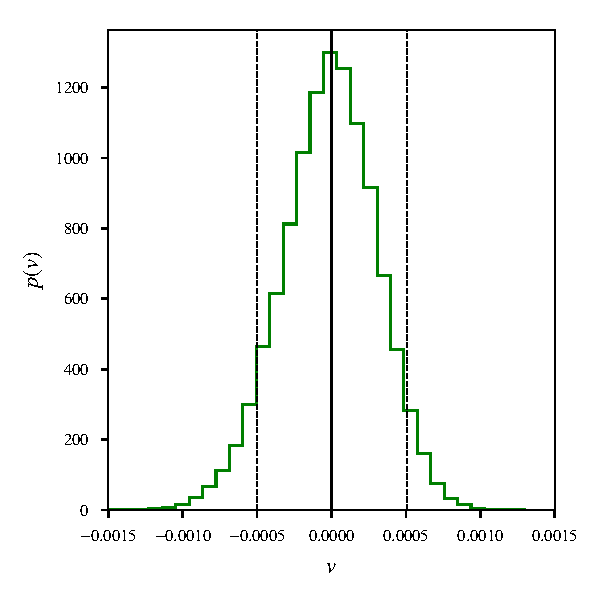
\includegraphics[scale=0.7]{figs/v1_GR_hist_M_80_q_9_dL_250.pdf} 
    \end{center} 
    \caption{Histogram of the deviation parameter $v$ estimated from simulated GR signal for binaries with $M=80$ $M_{\odot}$ and $q=1/9$. SNR fixed at 100.}
    \label{fig:cs_hist}
\end{figure}


\begin{figure}[h]
    \begin{center}
    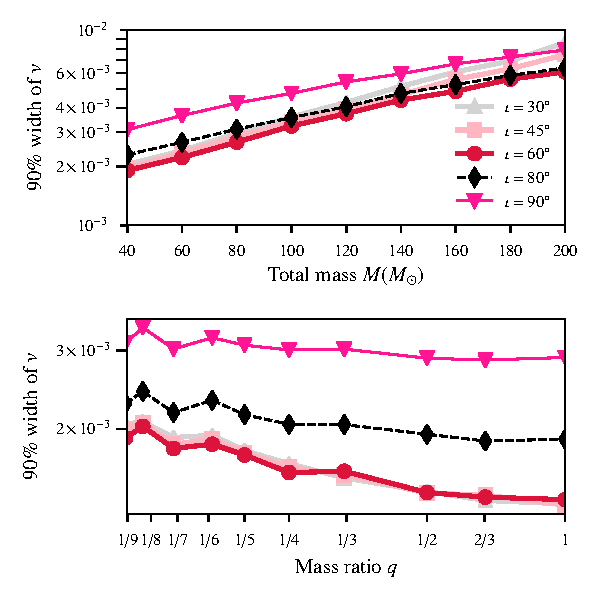
\includegraphics[scale=0.75]{figs/v1_confidence_interval_pol.pdf} 
    \end{center} 
    \caption{The plots shows the width of the 90\% credible region of the deviation parameter $v_1$ estimated from different polarizations of simulated GR signals for binaries with different total mass $M$ and mass ratio $q$. All binaries correspond to a SNR 25.}
    \label{fig:cs_bound}
\end{figure}

\newpage
\begin{figure}[h!]
    \begin{center}
    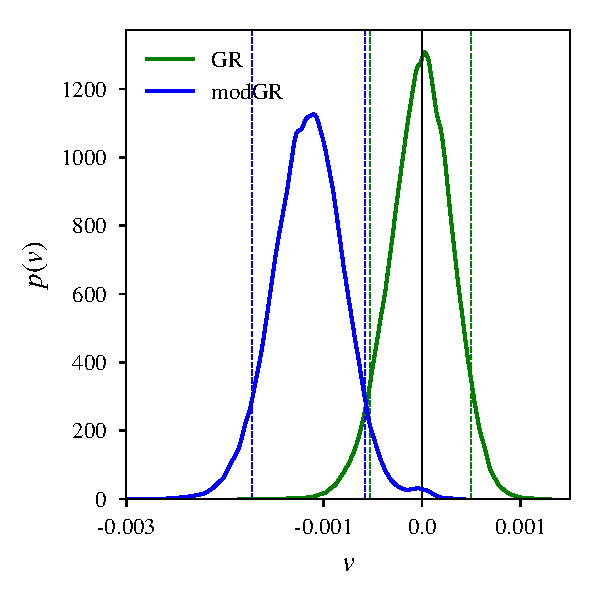
\includegraphics[scale=0.7]{figs/v1_modgr_hist_M_80_q_9_dL_250.pdf} \end{center} 
    \caption{Histograms of the deviation parameter $v$ estimated from simulated GR and modGR signal for binaries with $M=80$ $M_{\odot}$, $q=1/9$ and $dL=200$ Mpc.}
    \label{fig:cs_modgr}
\end{figure}

\bibliographystyle{apsrev-nourl}
\bibliography{TestGR.bib}

\end{document}
